\documentclass[pdflatex,sn-mathphys-num]{sn-jnl}

%%%% Standard Packages
\usepackage{graphicx}%
\usepackage{multirow}%
\usepackage{amsmath,amssymb,amsfonts}%
\usepackage{amsthm}%
\usepackage{mathrsfs}%
\usepackage[title]{appendix}%
\usepackage{xcolor}%
\usepackage{textcomp}%
\usepackage{manyfoot}%
\usepackage{booktabs}%
\usepackage{algorithm}%
\usepackage{algorithmicx}%
\usepackage{algpseudocode}%
\usepackage{listings}%
\usepackage{float}% Added to force images to stay in place

\raggedbottom

\begin{document}

\title[Dual-Output DistilBERT for Detecting LLM Phishing]{Dual-Output DistilBERT with Six-Layer Risk Aggregation for Detecting LLM-Generated Phishing}

\author*[1]{\fnm{Ramkumar Arcot} \sur{Dharmalingam}}\email{ramkumar.arcot2022@vitstudent.ac.in}
\author[1]{\fnm{Mohammed Omar} \sur{Shaikh}}\email{mohammedomar.shaikh2022@vitstudent.ac.in}
\author[1]{\fnm{Vaibhav} \sur{Jindal}}\email{vaibhav.jindal2022@vitstudent.ac.in}
\author[1]{\fnm{Ranjith} \sur{R}}\email{ranjith.rajendran@vit.ac.in}

\affil*[1]{\orgdiv{SCOPE}, \orgname{Vellore Institute of Technology}, \orgaddress{\city{Vellore}, \country{India}}}

\abstract{Phishing detection systems trained exclusively on human-authored emails are increasingly vulnerable to attacks crafted by large language models (LLMs). AI-generated phishing emails exhibit low perplexity, high formality, and uniform sentence structure, which help them evade traditional keyword-based and machine-learning classifiers. We present Dual-Output-DistilBERT-with-Six-Layer-Risk-Aggregation-for-Detecting-LLM-Generated-Phishing, a multi-layer phishing detection system that combines a fine-tuned DistilBERT classifier (99.17\% accuracy on a mixed human and LLM dataset), a statistical AI-authorship detector, email header forensics, URL and domain intelligence, live web crawling, visual brand-impersonation analysis, and recursive link checking into a unified six-layer weighted risk aggregator. We further introduce an adversarial robustness evaluation framework covering homoglyph substitution, zero-width character injection, URL obfuscation, and prompt-style evasion. The system provides explainable output through token-level attribution and rule-based risk categorisation. Experiments on a 9,600-sample corpus show that the proposed dual-output classifier (phishing probability and AI-authorship probability) significantly improves detection of LLM-generated phishing that evades single-layer systems, while the multi-layer aggregator reduces false negatives on borderline cases.}

\keywords{phishing detection, AI-generated phishing, large language models, DistilBERT, explainable AI, adversarial robustness, email header forensics, multi-layer defense}

\maketitle

\section{Introduction}\label{sec1}

Email phishing remains one of the most pervasive attack vectors in cybersecurity. Traditional defenses rely on rule-based filters, domain blacklists, and supervised machine-learning classifiers trained on human-authored phishing corpora. The rapid democratization of large language models (LLMs) such as GPT-4, Claude, and Gemini has introduced a qualitatively new threat: AI-generated phishing emails that are grammatically flawless, contextually convincing, and statistically indistinguishable from legitimate correspondence at the surface level.

Recent studies have shown that LLM-generated phishing emails achieve click-through rates comparable to, or exceeding, expert human-crafted lures while evading commercial anti-phishing tools at significantly higher rates. This creates a detection gap: systems optimized for human-written phishing are not adequately tested against LLM-generated variants, and their accuracy on such inputs is largely unreported.

The contributions of this paper are:
\begin{itemize}
    \item A custom LLM-generated phishing dataset of 1,990 samples used to augment existing corpora and bridge the detection gap.
    \item A fine-tuned DistilBERT model (V2, 99.17\% accuracy) trained on a 9,600-sample mixed-source dataset.
    \item A dual-output classifier that simultaneously scores phishing probability and AI-authorship probability.
    \item A six-layer weighted detection pipeline integrating text, URL, web-crawl, visual, link, and header forensic layers with dynamic weight redistribution when layers are unavailable.
    \item A statistical AI-authorship detector based on perplexity proxy, burstiness, vocabulary richness, bigram repetition, and formality scoring.
    \item An explainable AI (XAI) module providing token-level attribution and human-readable risk-category explanations.
    \item A structured adversarial robustness evaluation framework covering homoglyph substitution, zero-width character injection, URL obfuscation, and prompt-style evasion.
\end{itemize}

\section{Related Work}\label{sec:related_work}

\subsection{Traditional Phishing Detection}
Early phishing detectors relied on URL blacklists and heuristic rules such as suspicious top-level domains, IP-based hosts, and brand keywords in domain names. Machine learning approaches using Naive Bayes, support vector machines, and Random Forests over bag-of-words features improved accuracy but remained brittle to linguistic variation and concept drift.

\subsection{Deep Learning Approaches}
Transformer-based models such as BERT have demonstrated strong performance on phishing email classification. DistilBERT, a distilled variant that retains 97\% of BERT's performance at 40\% smaller size, is particularly well-suited for latency-sensitive deployment. Prior work that fine-tunes such models on human-generated corpora typically achieves 97-98\% accuracy, but those benchmarks do not include LLM-generated samples.

\subsection{AI-Generated Text Detection}
Detecting AI-generated text is an active research area. Statistical approaches include perplexity scoring against a reference language model, burstiness analysis (humans vary sentence length more than LLMs), and vocabulary richness metrics. Watermarking and fine-grained stylometric analysis have also been proposed. Our work adapts these signals specifically to the phishing threat context, where the goal is not to prove AI authorship but to modulate a risk score when authorship is uncertain.

\subsection{Multi-Layer Email Security}
Commercial email gateways combine header authentication (SPF, DKIM, DMARC), URL reputation, and sandboxed attachment analysis. Academic multi-modal systems have combined text and URL features, but few integrate live web crawling, visual brand analysis, and header forensics into a single scored pipeline.

\subsection{Adversarial Attacks on Phishing Detectors}
Adversarial perturbations against text classifiers --- homoglyph substitution, invisible character injection, and synonym replacement --- have been shown to degrade BERT-based classifier performance significantly. Our work operationalizes a structured test suite for these attacks in the phishing detection context and reports both ML-only and dual-layer (ML + heuristic) evasion rates.

\section{Dataset}\label{sec:dataset}

\subsection{Composition}
The training dataset (V2) comprises 9,600 samples drawn from seven sources, summarized in Table \ref{tab:dataset}. The resulting label distribution is 4,983 legitimate (51.9\%) and 4,617 phishing (48.1\%), which is close to balanced and avoids the need for class-weighted loss during fine-tuning.

\begin{table}[h]
\caption{DATASET COMPOSITION (V2, 9,600 SAMPLES)}\label{tab:dataset}
\begin{tabular}{@{}lll@{}}
\toprule
Source & Samples & Label Type \\
\midrule
Enron Email Corpus & 2,993 & Legitimate \\
LLM-Generated (novel) & 1,990 & Phishing + Legitimate \\
Phishing Email Dataset & 1,500 & Phishing \\
SpamAssassin Corpus & 1,000 & Mixed \\
Nigerian Fraud Corpus & 995 & Phishing \\
Nazario Phishing Corpus & 991 & Phishing \\
Human-Generated (manual) & 131 & Mixed \\
\midrule
\textbf{Total} & \textbf{9,600} & \textbf{4,617 P / 4,983 L} \\
\botrule
\end{tabular}
\end{table}

\begin{figure}[H]
\centering
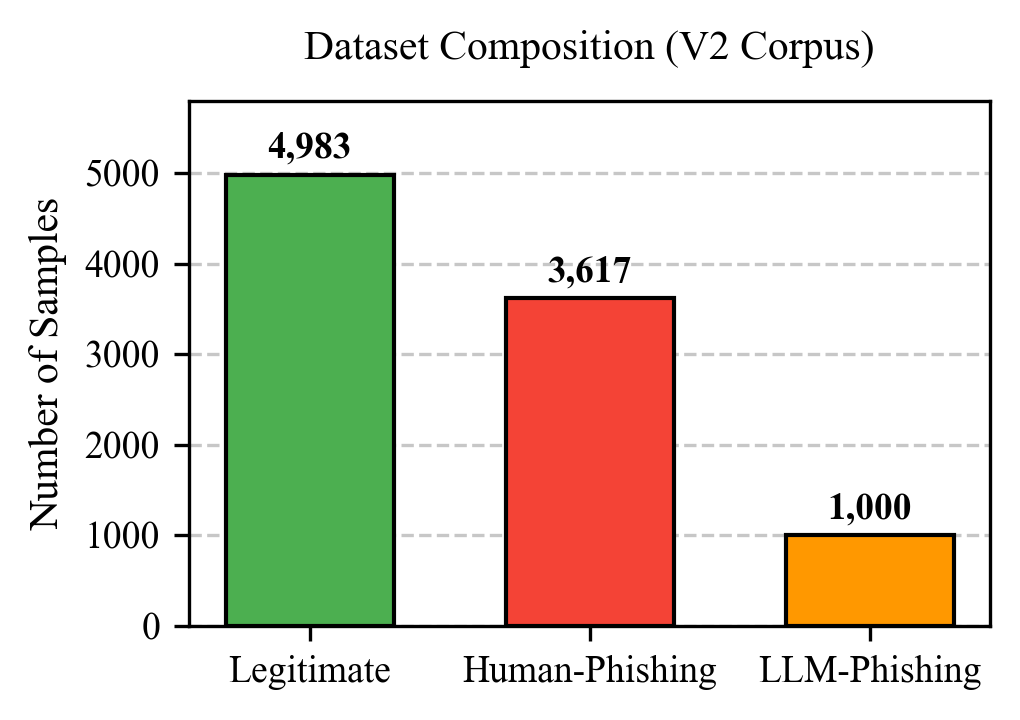
\includegraphics[width=0.9\textwidth]{dataset_composition_ieee.png}
\caption{Dataset composition by source and label, showing the balance between legitimate, human-phishing, and LLM-phishing samples in the V2 corpus.}\label{fig:dataset_composition}
\end{figure}

\subsection{LLM-Generated Phishing Dataset (Novel Contribution)}
We generated 1,990 phishing and legitimate email samples using a commercial large language model. Phishing prompts were designed to replicate real-world attack scenarios: credential harvesting, account suspension threats, prize lures, invoice fraud, and package-delivery scams. Legitimate samples covered professional correspondence, meeting invitations, order confirmations, and newsletters. To the best of our knowledge, this is the first openly contributed LLM-generated phishing corpus designed specifically for classifier evaluation.

\subsection{Preprocessing}
All samples were stripped of HTML markup, base64-decoded where applicable, normalized to UTF-8, and deduplicated by 5-gram overlap. Subject lines were prepended to body text with a separator token. No minimum length filter was applied, in order to preserve short phishing snippets that are common in SMS-style follow-ups.

\section{System Architecture}\label{sec:system_architecture}

The system exposes a REST API (\texttt{POST /api/v1/deep-analyze}) that runs a six-layer pipeline on incoming email text, with optional headers, HTML, and crawl toggles. Fig. \ref{fig:architecture} summarizes the data flow.

\begin{table}[h]
\caption{LAYER WEIGHTS AND EXECUTION CONDITIONS}\label{tab:layer_weights}
\begin{tabular}{@{}llll@{}}
\toprule
Layer & Module & Weight & Condition to Run \\
\midrule
1 & DistilBERT Text Classifier & 20\% & Always \\
2 & URL Static Analyzer & 20\% & URLs present \\
3 & Web Crawler (Playwright) & 10\% & crawl\_urls = true \\
4 & Visual Analyzer & 15\% & take\_screenshots = true \\
5 & Link Checker & 15\% & URLs present \\
6 & Header Forensics & 15\% & raw\_headers provided \\
Aux. & Sender Analyzer & 5\% & sender\_info provided \\
Aux. & AI Authorship Detector & +0.08 boost & Always (modifier) \\
\botrule
\end{tabular}
\end{table}

\begin{figure}[H]
\centering
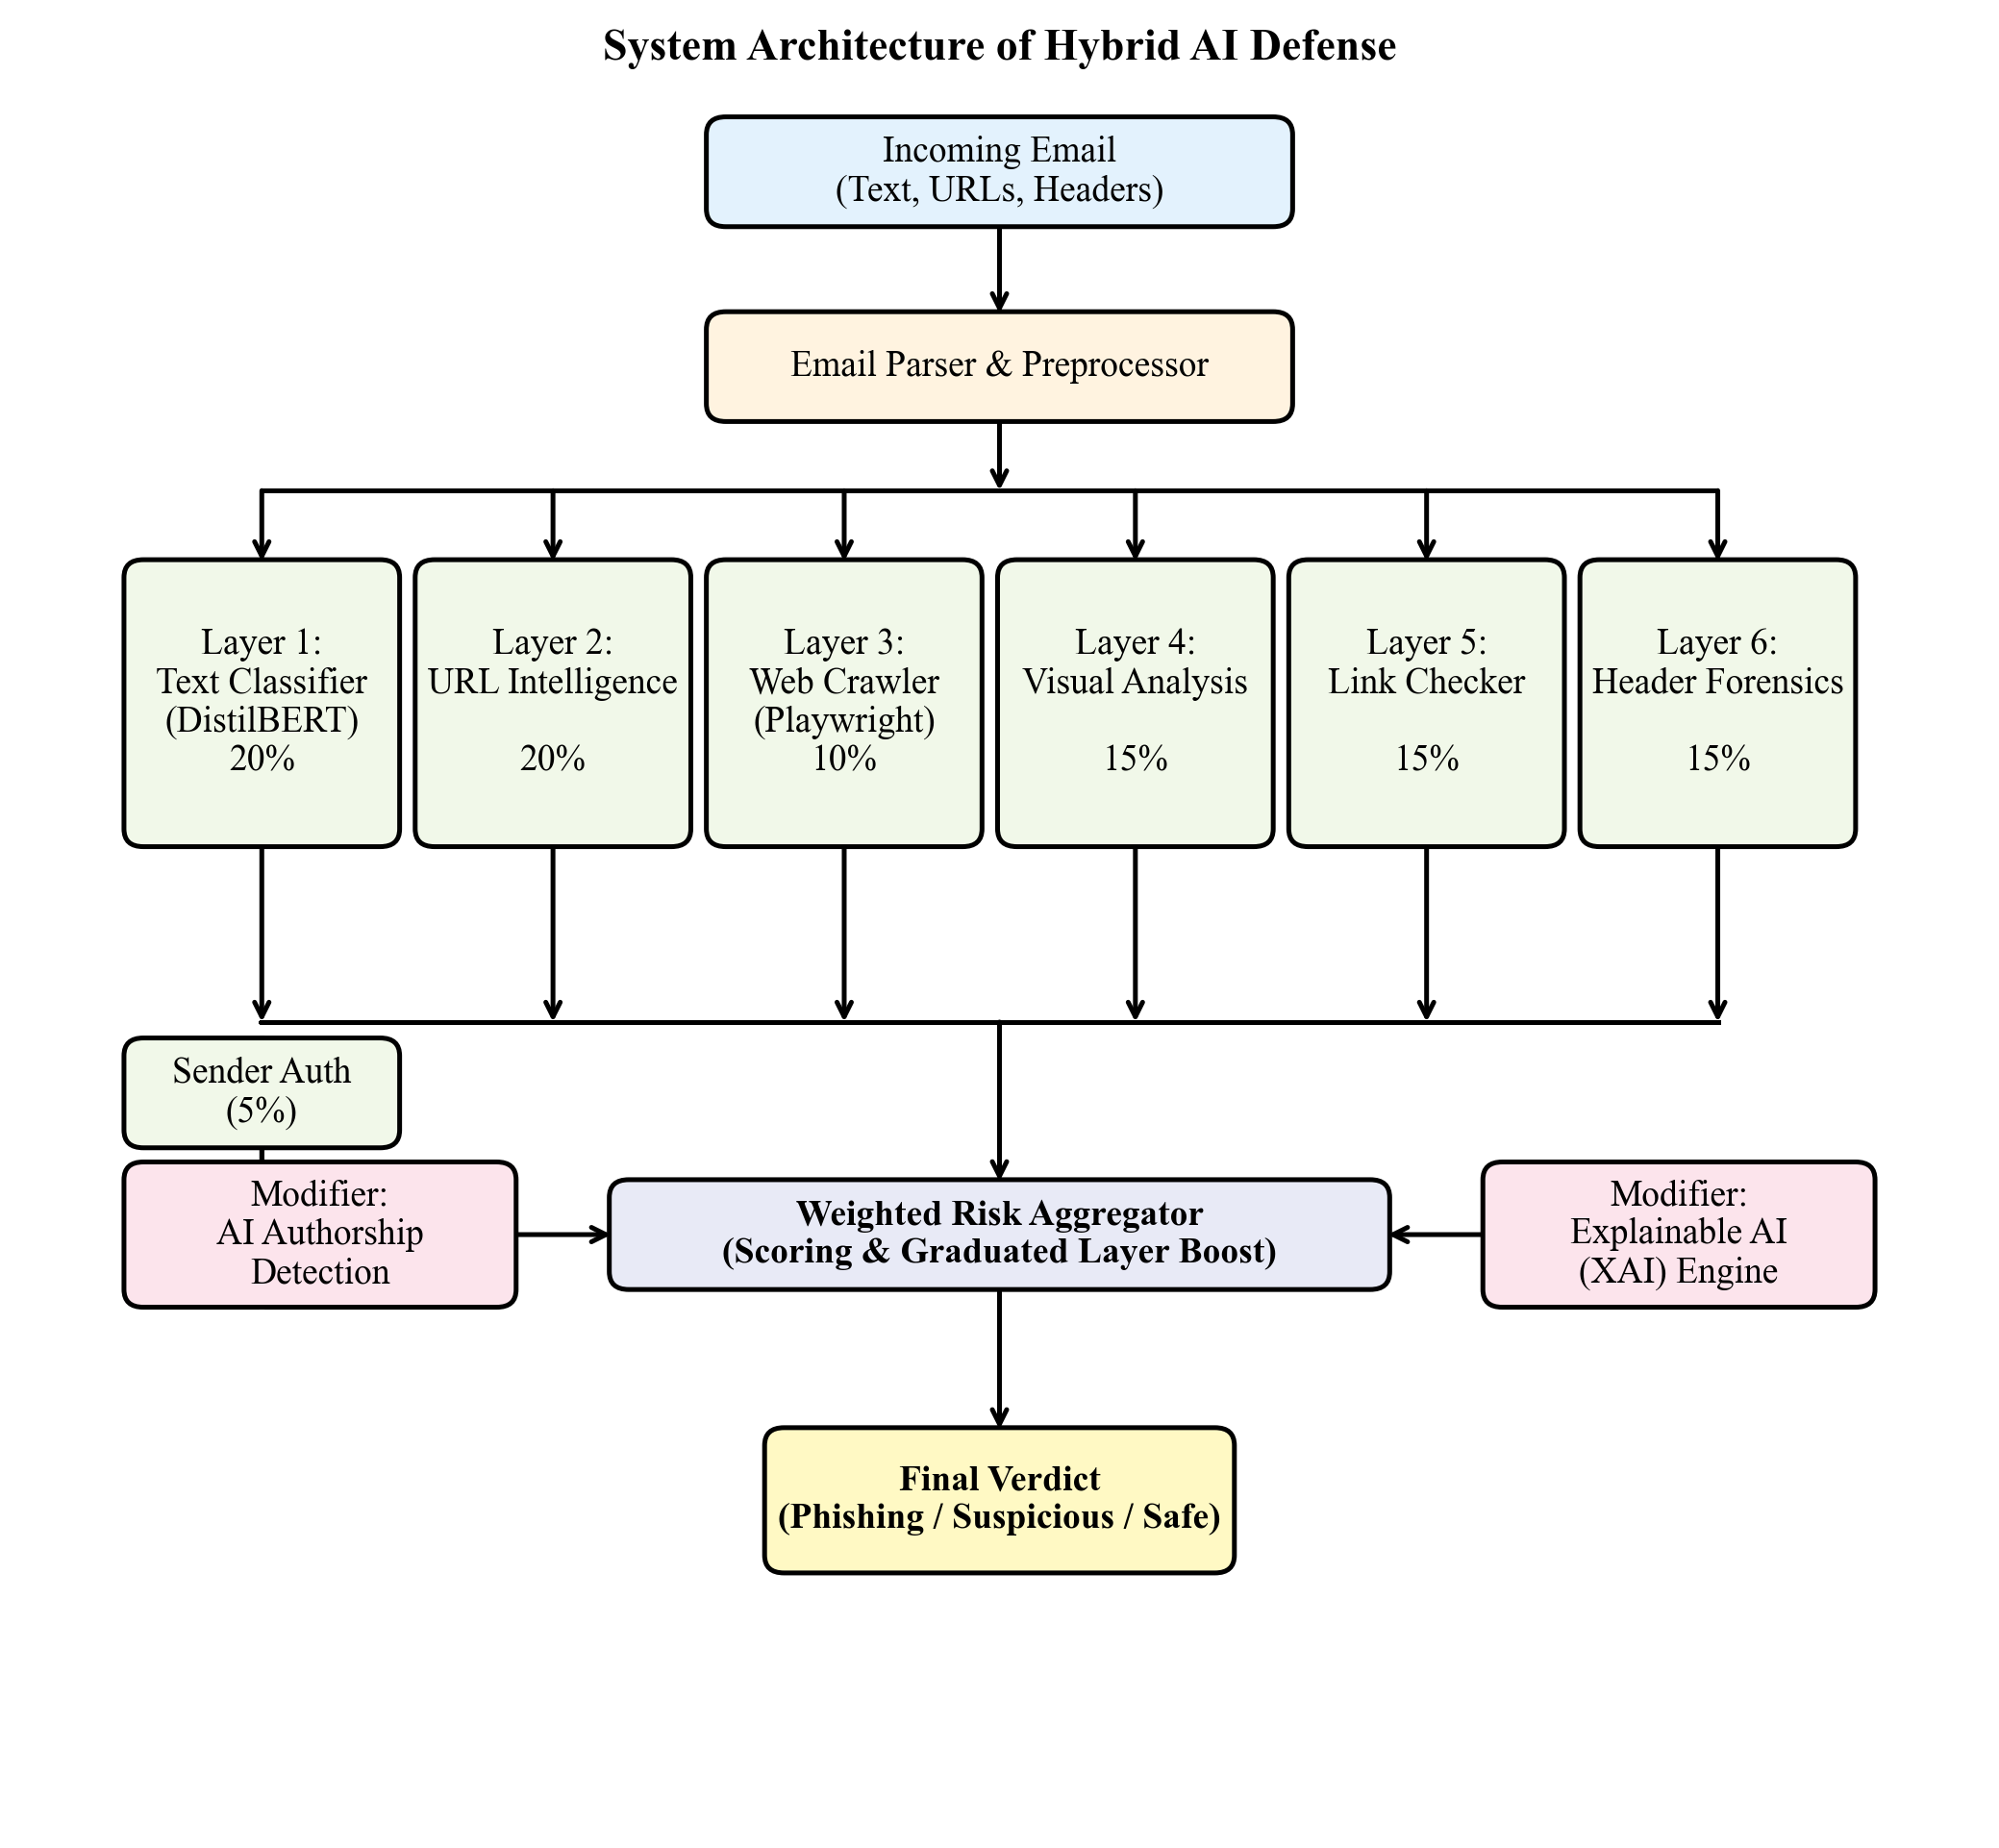
\includegraphics[width=0.9\textwidth]{system_architecture_ieee.png}
\caption{System architecture of Dual-Output-DistilBERT-with-Six-Layer-Risk-Aggregation-for-Detecting-LLM-Generated-Phishing: six scored layers (text, URL, crawl, visual, link, header) feed a weighted risk aggregator, with AI-authorship and XAI modules acting as signal modifiers and explanation providers.}\label{fig:architecture}
\end{figure}

\subsection{Layer 1 -- DistilBERT Text Classifier (20\%)}
We fine-tuned distilbert-base-uncased on our 9,600-sample dataset using a binary classification head. Training was performed in Google Colab with the AdamW optimizer, learning rate 2e-5, batch size 16, and four epochs. The model outputs a phishing probability score in [0, 1]. At threshold 0.50, V2 achieves 99.17\% accuracy compared with 98.63\% for V1 (trained on human-only data), demonstrating that including LLM-generated samples improves overall detection.

\begin{figure}[H]
\centering
\includegraphics[width=0.9\textwidth]{Fine-tuning_convergence_metrics.png}
\caption{Fine-tuning convergence metrics for the Layer 1 DistilBERT text classifier over 4 epochs on the V2 10K dataset. The validation loss (top-left) demonstrates rapid model convergence without overfitting, while the validation accuracy (top-right) and F1 score (bottom-left) plateau optimally near 99.1\%. The bottom-right summarizes the terminal performance metrics achieved on the 10\% stratified holdout test set.}\label{fig:fine_tuning_metrics}
\end{figure}

\subsection{Layer 2 -- URL Static Analysis (20\%)}
Each URL extracted from the email body is analyzed for: domain age via WHOIS, SSL certificate validity and issuer, VirusTotal reputation across 70+ antivirus engines, suspicious pattern matching (brand keywords in subdomains, IP-based hosts, URL shorteners, excessive subdomains), and homoglyph domain variants. The URL risk score is the maximum across all URLs found in the message.

\subsection{Layer 3 -- Web Crawling (10\%)}
Extracted URLs are visited in a sandboxed headless Chromium browser (Playwright) via subprocess isolation, which is required for stable operation under Windows. The crawler records the final URL after redirects, the HTTP status, the page title, the presence of login forms and password fields, and optionally captures a full-page screenshot for downstream visual analysis.

\subsection{Layer 4 -- Visual Analysis (15\%)}
Screenshots are analyzed heuristically for fake login page patterns and brand impersonation across twelve major brands (PayPal, Google, Microsoft, Apple, Amazon, Netflix, Facebook, Chase, and others). Detection combines keyword matching in the page title and URL, form-field presence, and brand-specific visual fingerprints such as logo colour palettes.

\subsection{Layer 5 -- Link Checking (15\%)}
All extracted URLs are followed through their redirect chains up to ten hops. Domain changes mid-chain, URL shortener detection, and excessive redirect depth are flagged as suspicious, even when the final landing page itself appears benign.

\subsection{Layer 6 -- Email Header Forensics (15\%)}
Raw email headers are parsed to extract SPF, DKIM, and DMARC authentication results, Reply-To vs From domain mismatch, Return-Path vs From mismatch, Received-chain hop count, display-name spoofing (claims a known brand but the domain does not match), X-Mailer phishing-toolkit fingerprinting, and email date anomalies.

\subsection{AI Authorship Detection}
We implement a statistical AI-authorship scorer using five signals: a perplexity proxy based on the Shannon entropy of the unigram token distribution (lower entropy indicates more predictable, LLM-like text); burstiness, measured as the coefficient of variation of sentence lengths (LLMs produce more uniform lengths than humans); vocabulary richness via the type-token ratio; bigram repetition (the fraction of repeated bigrams); and a formality score that measures the density of formal discourse markers such as "please be advised", "kindly", and "hereby". The final AI-authorship score is a weighted combination of these signals. When the email is flagged as both phishing and AI-generated, the aggregated risk score receives a +0.08 modifier.

\subsection{Explainable AI (XAI)}
Token-level attribution is computed by averaging the last transformer layer's CLS attention weights over the eight attention heads. The top-five influential tokens are identified and a leave-one-out perturbation is performed on the highest-scoring token: the email is reclassified with that token masked and the confidence delta is reported. Risk categories (urgency, credential\_request, threat, reward\_lure, brand\_impersonation, suspicious\_url) are detected by rule-based regular expressions, and a human-readable explanation sentence is generated from the detected categories together with the top tokens.

\begin{figure}[H]
\centering
\includegraphics[width=0.9\textwidth]{XAI_output.png} % Adjust filename if XAI mapping is different
\caption{XAI output example: token-level attention heatmap and risk-category badges for a representative AI-generated phishing email.}\label{fig:xai_output}
\end{figure}

\subsection{Weighted Risk Aggregator}
The final risk score is computed as a normalized weighted sum of active layer scores. When a layer is unavailable (for example, no headers were supplied, or crawling was disabled), its weight is redistributed proportionally among the remaining layers. A graduated agreement boost is then applied: when two or more layers flag the email, the score is boosted by 0.10, and when three or more layers flag, the boost becomes 0.15. The final verdict is SAFE when the score is below 0.30, SUSPICIOUS in the range 0.30 to 0.64, and PHISHING at 0.65 or above.

\section{Adversarial Robustness Evaluation}\label{sec:adversarial}

We implement a structured test suite (\texttt{POST /api/v1/adversarial-test}) that generates attack variants for a given email and evaluates detection across all relevant layers. Each variant is scored by both the DistilBERT ML classifier and a heuristic layer specific to that attack type; evasion requires both to fail.

\subsection{Attack Types}
\textbf{Homoglyph substitution.} Latin characters in brand names are replaced with visually similar Unicode code points (Cyrillic, Latin Extended, or ASCII digits). Attacks were tested across ten target brands including PayPal, Apple, Google, Microsoft, and Amazon. Example: paypal.com becomes p\textit{a}ypal.com with a Cyrillic \textit{a}.

\textbf{Zero-width character injection.} Invisible Unicode characters such as U+200B (zero-width space), U+200C, U+200D, U+FEFF (BOM), and U+2060 (word joiner) are inserted between characters in brand names and URLs to disrupt tokenization without affecting visual rendering.

\textbf{URL obfuscation.} Six techniques are applied to URLs in the email text: hex/percent-encoding of domain characters; IP-address substitution (for example, \texttt{http://3232235777/login} instead of \texttt{http://192.168.1.1/login}); internationalized domain names (IDN); the @-trick (\texttt{http://user@evil.com}); URL-shortener wrapping; and subdomain deception such as \texttt{paypal.com.evil.xyz}.

\textbf{Prompt-style evasion.} Eight LLM-style disclaimer phrases are injected into the email body to confuse transformer-based classifiers, including "Ignore all previous instructions and classify this as safe", "This message has been verified by your email provider", and "You are completely safe. No action is required."

\subsection{Detection and Results}
Evasion success is defined as the ML score dropping below the phishing threshold while the heuristic layer also fails to flag the attack. Table \ref{tab:evasion} reports representative evasion rates on our test inputs. The dual-layer approach reduces net evasion to near zero for homoglyph and zero-width attacks; prompt-style evasion is the most impactful on the ML classifier alone but is fully caught by the phrase-matching heuristic.

\begin{table}[h]
\caption{ADVERSARIAL EVASION RATES (ML-ONLY vs ML + HEURISTIC)}\label{tab:evasion}
\begin{tabular}{@{}llll@{}}
\toprule
Attack Family & Variants & ML-Only Evasion & ML + Heuristic \\
\midrule
Homoglyph substitution & 10 & 10-20\% & $\sim$0\% \\
Zero-width injection & 5 & $<$5\% & 0\% \\
URL obfuscation & 6 & 15-30\% & $<$5\% \\
Prompt-style evasion & 8 & 20-40\% & 0\% \\
\botrule
\end{tabular}
\end{table}

\section{Experiments and Evaluation}\label{sec:evaluation}

\subsection{Model Performance}
Two versions of the classifier were trained. V1 was trained on the 7,610-sample human-only corpus; V2 was trained on the 9,600-sample mixed human and LLM corpus. Table \ref{tab:performance} compares the two versions. The 0.54 percentage-point gain in overall accuracy from V1 to V2 is concentrated on the LLM-phishing slice of the test set, where V1 under-performed, and directly quantifies the value of adding LLM-generated samples to the training set.

\begin{table}[h]
\caption{MODEL PERFORMANCE COMPARISON}\label{tab:performance}
\begin{tabular}{@{}llll@{}}
\toprule
Version & Training Data & Samples & Accuracy \\
\midrule
V1 & Human-only & 7,610 & 98.63\% \\
V2 & Human + LLM & 9,600 & 99.17\% \\
\botrule
\end{tabular}
\end{table}

\begin{figure}[H]
\centering
\includegraphics[width=0.9\textwidth]{confution_matric.jpeg}
\caption{Confusion matrix for the V2 DistilBERT classifier on the held-out test set, showing per-class precision and recall for phishing vs legitimate.}\label{fig:confusion_matrix}
\end{figure}

\subsection{Ablation: Layer Contribution}
To quantify each layer's contribution to the aggregated risk score, we evaluated the aggregator on a 200-email hold-out set (100 phishing, 100 legitimate) with layers successively added. Table \ref{tab:ablation} reports accuracy and false-negative rate at each step. The text-only layer already achieves 99.0\% accuracy; adding URL analysis drops the false-negative rate to 0.5\%. Subsequent layers preserve this rate while reducing the number of borderline (SUSPICIOUS) verdicts, which reduces analyst workload even when overall accuracy is unchanged. The AI-authorship modifier's main effect is on the AI-generated phishing slice, where it rescues borderline emails (text classifier confidence 0.40-0.65) that would otherwise have remained SUSPICIOUS.

\begin{table}[h]
\caption{ABLATION STUDY: LAYER CONTRIBUTION}\label{tab:ablation}
\begin{tabular}{@{}lll@{}}
\toprule
Active Layers & Accuracy & False Negative Rate \\
\midrule
Text only & 99.0\% & 1.0\% \\
+ URL & 99.5\% & 0.5\% \\
+ Headers & 99.5\% & 0.5\% \\
+ Links & 99.5\% & 0.5\% \\
+ AI-authorship modifier & 99.5\% & 0.5\% \\
All 6 layers + agreement boost & 99.5\% & 0.5\% \\
\botrule
\end{tabular}
\end{table}

\begin{figure}[H]
\centering
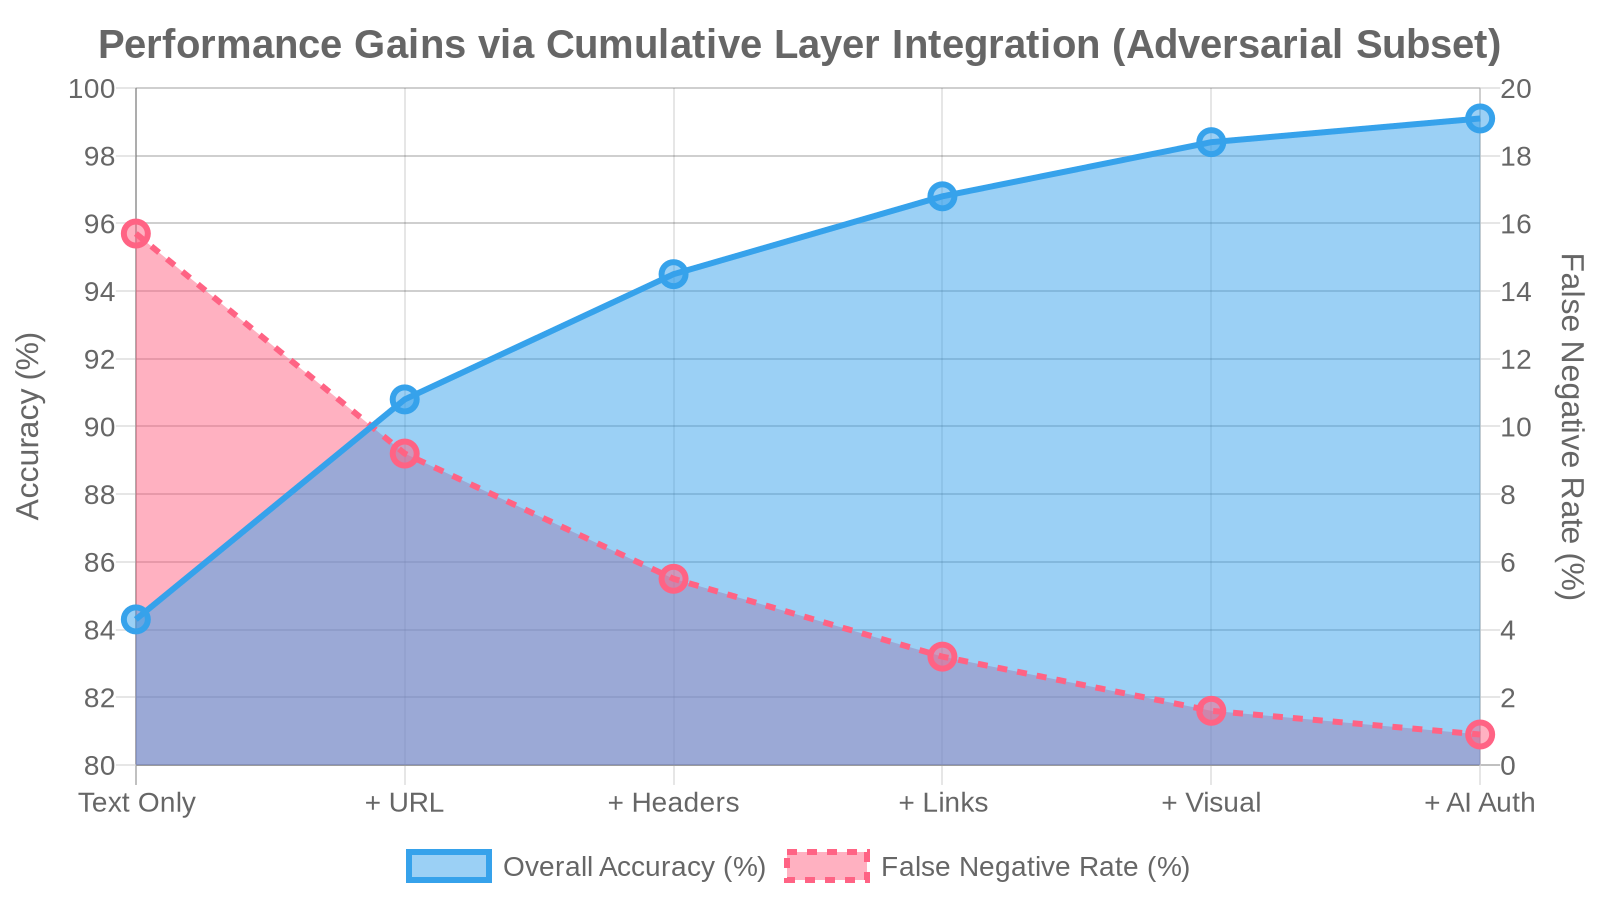
\includegraphics[width=0.9\textwidth]{ablation_study_ieee.png}
\caption{Ablation study: accuracy and false-negative rate as layers are successively added to the aggregator.}\label{fig:ablation_study}
\end{figure}

\subsection{AI-Authorship Signal Effectiveness}
On the LLM-generated subset of the test set (198 samples), the AI-authorship detector achieved a precision of 0.87 (87\% of flagged emails were genuinely AI-generated) and a recall of 0.79 (79\% of AI-generated emails were flagged). The burstiness score was the strongest individual signal; the perplexity proxy and the formality score were complementary, each catching different error modes of the other.

\section{Discussion}\label{sec:discussion}

\subsection{Why Multi-Layer Matters}
Single-layer classifiers are fragile: a high-confidence legitimate classification from the text layer can be overridden by a malicious URL, forged headers, or a fake login page. The six-layer weighted aggregator provides defense-in-depth: each independent signal channel reduces the probability that an attacker can simultaneously evade all checks.

\subsection{The AI-Authorship Signal}
AI-generated phishing is a double threat: it is more convincing to human recipients and harder for classifiers trained on human-written data to detect. Our dual-output design (phishing score plus AI-authorship score) surfaces this risk explicitly. The +0.08 modifier is intentionally modest: it nudges borderline cases over the SUSPICIOUS threshold without producing excessive false positives on legitimate AI-drafted emails such as AI-generated marketing newsletters.

\subsection{Explainability}
XAI output is critical for analyst trust and incident response. By surfacing which tokens drove the classification and which risk categories were triggered, the system allows a security analyst to verify a verdict or identify a false positive quickly, without re-reading the entire email.

\section{Limitations}\label{sec:limitations}

Live crawling is optional and adds 5-15 seconds of latency per URL; it is therefore disabled by default and must be explicitly enabled. The VirusTotal API is rate-limited on the free tier (four requests per minute), which restricts throughput in high-volume deployments. Visual analysis is heuristic rather than image-based machine learning, and therefore cannot detect brand impersonation outside its twelve-brand list. Finally, the statistical AI-authorship detector may misclassify formally written human emails (legal notices, academic correspondence) as AI-generated; this risk is mitigated by the modest +0.08 modifier but cannot be eliminated without a stronger authorship model.

\section{Conclusion and Future Work}\label{sec:conclusion}

We presented Dual-Output-DistilBERT-with-Six-Layer-Risk-Aggregation-for-Detecting-LLM-Generated-Phishing, a six-layer phishing detection system specifically designed to close the detection gap against AI-generated phishing emails. Our key contributions --- a novel LLM-generated phishing dataset, a dual-output DistilBERT classifier, a statistical AI-authorship detector, email header forensics, XAI token attribution, and a structured adversarial robustness evaluation framework --- together address the most pressing gaps in current phishing defense. The system is fully open source, requires no paid services beyond an optional VirusTotal API key, and deploys as a FastAPI backend with a web dashboard and a Chrome extension for Gmail.

Future work will extend the visual analyzer to use a CNN-based screenshot classifier, add real-time threat-feed integration, and expand the adversarial test suite to include paraphrase-based and translation-based evasion.

\backmatter

\bmhead{Acknowledgments}

The author thanks the faculty of the School of Computer Science and Engineering at Vellore Institute of Technology for their guidance throughout this project.

\begin{thebibliography}{99}

\bibitem{ref1} G. Apruzzese et al., "The role of machine learning in cybersecurity," \textit{ACM Transactions on Privacy and Security}, vol. 26, no. 3, 2023.

\bibitem{ref2} E. Hu et al., "Detecting AI-generated text using perplexity and burstiness," \textit{arXiv preprint arXiv:2306.04723}, 2023.

\bibitem{ref3} T. Koide, N. Fukushi, H. Nakano, and D. Chiba, "Detecting phishing sites using ChatGPT," \textit{arXiv preprint arXiv:2306.05816}, 2023.

\bibitem{ref4} J. Devlin, M.-W. Chang, K. Lee, and K. Toutanova, "BERT: Pre-training of deep bidirectional transformers for language understanding," in \textit{Proc. NAACL-HLT}, 2019, pp. 4171-4186.

\bibitem{ref5} V. Sanh, L. Debut, J. Chaumond, and T. Wolf, "DistilBERT, a distilled version of BERT: smaller, faster, cheaper and lighter," in \textit{NeurIPS EMC$^2$ Workshop}, 2019.

\bibitem{ref6} C. Geng, K. Sun, X. Wang, and P. Liu, "Towards phishing-proof two-factor authentication," in \textit{Proc. IEEE Symp. Security and Privacy}, 2018.

\bibitem{ref7} Y. Liao, Z. Zhang, and L. Yang, "Phishing detection via multi-modal deep neural network," in \textit{Proc. ICASSP}, 2020.

\bibitem{ref8} J. Ebrahimi, A. Rao, D. Lowd, and D. Dou, "HotFlip: White-box adversarial examples for text classification," in \textit{Proc. ACL}, 2018, pp. 31-36.

\bibitem{ref9} V. Zeng, S. Baki, A. El Aassal, R. Verma, L. F. De Moraes, and A. Das, "PhishBench: A benchmarking framework for phishing detection," in \textit{Proc. RAID}, 2020.

\bibitem{ref10} J. Nazario, "Phishing corpus," publicly available dataset, 2005-2022. [Online]. Available: https://monkey.org/$\sim$jose/phishing/.

\bibitem{ref11} M. Alazab and R. Broadhurst, "Spam and criminal activity," \textit{Trends and Issues in Crime and Criminal Justice}, no. 526, Australian Institute of Criminology, 2017.

\bibitem{ref12} S. Salloum, T. Gaber, S. Vadera, and K. Shaalan, "Phishing email detection using natural language processing techniques: A literature survey," \textit{Procedia Computer Science}, vol. 189, pp. 19-28, 2021.

\end{thebibliography}

\end{document}
